% Updated 2024-11-26 23.37 
% source: Climate modeling notes ONLY CAP1

\chapter{Fundamental processes}
Different climate models incorporate all the complex physical processes occurring in the climate system using a variety of methods. The dynamic involves interactions between motions, thermodynamics, and atmospheric water content.

\section{Radiation}
The radiation that heats and cools the climate system can be divided into two parts: solar radiation (shortwave) and terrestrial radiation (longwave).
All gases emit and absorb radiation, and each chemical element or combination of elements has a distinct spectrum indicating at which electromagnetic wavelengths its emissions occur. In some cases, the emission may be confined to narrow portions of the electromagnetic spectrum rather than being a smoothly varying function of wavelength. This phenomenon of distinct, discrete emission spectra results from the emission of radiation as an electron moves from one orbit around an atomic nucleus to another orbit closer to the nucleus. If the atom is excited by absorbing energy, then the electron can go to a higher (outer) discrete orbit.
As electrons return to the inner orbits, emission occurs in the ultraviolet part of the spectrum, producing the emission spectra. As electrons return instead from higher orbits to intermediate orbits, the emission is in the visible part of the spectrum; for the outer orbits, the emission is in the infrared.
Suppose radiational energy enters an atomic or molecular gas and is absorbed. In that case, it can increase the atomic or molecular energy levels by the same amount of energy involved in the emission. This absorption can be just as discrete or selective as the emission. Thus, if radiation entering a gas cannot excite the atoms or molecules in any energy form, then the radiational energy will not be absorbed or emitted in the gas. In the Earth's atmosphere, ozone, carbon dioxide, and water vapor are very important triatomic molecules that both emit and absorb radiation in certain parts of the electromagnetic spectrum that affect the climate system.

\begin{figure}[h!]
	\centering
	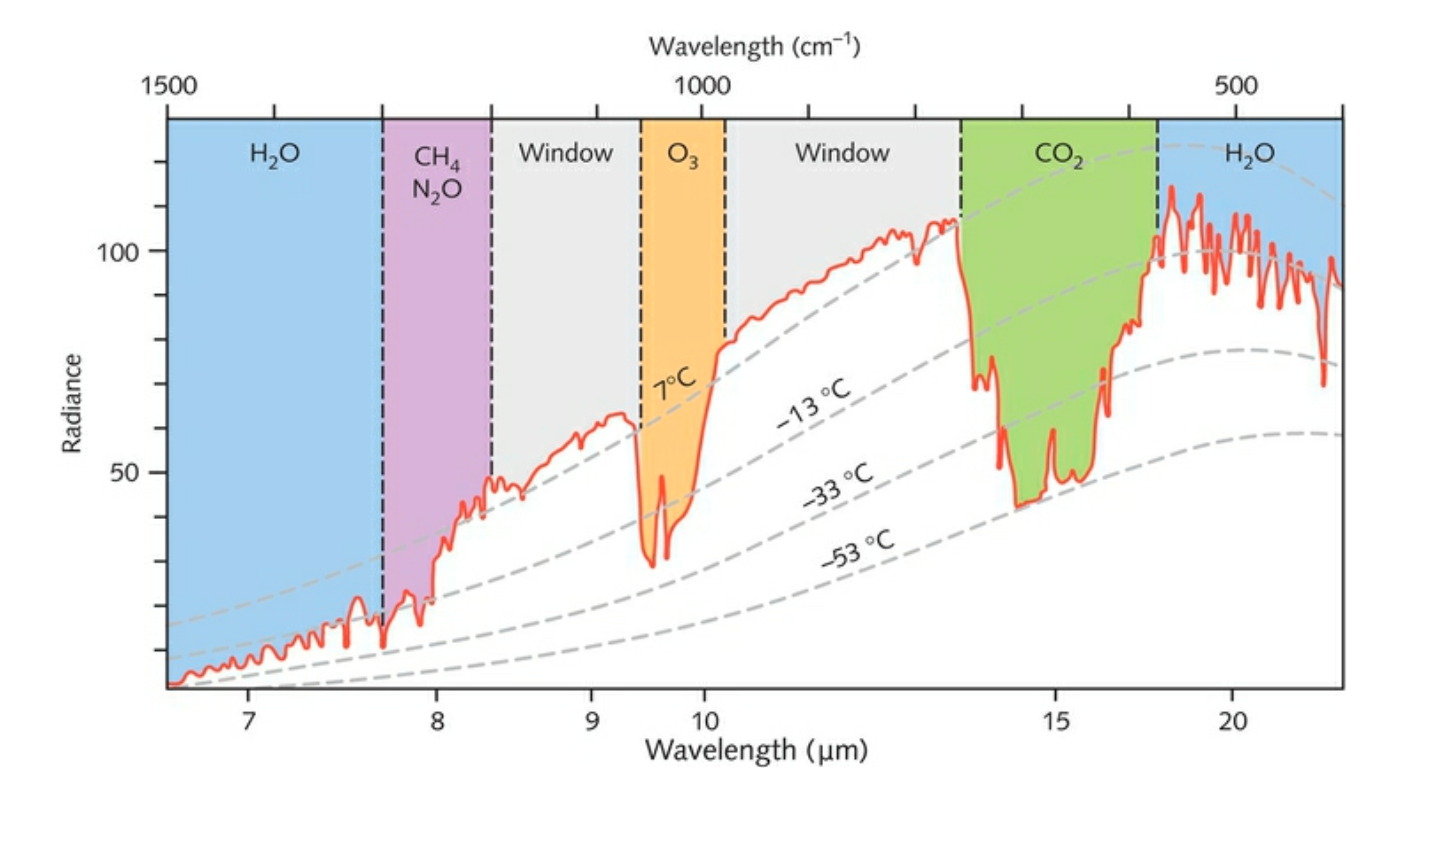
\includegraphics[width=0.5\linewidth]{uploads/image10.png}
	\caption{Earth's spectrum}
	\label{fig:enter-label}
\end{figure}
As we can see in figure \ref{fig:enter-label} ozone is a very strong absorber in the 9-10 µm region, carbon dioxide has absorption maxima in the 2, 3, 4, and 13-17 µm regions, and water vapor has several absorption regions in the 1-8 µm range and at wavelengths greater than 13 µm.

The radiational heating and cooling computation in climate models is usually done by calculating upward and downward fluxes through unit horizontal areas, considering the vertical distributions of temperature, water vapor, and other radiative absorbing gases such as carbon dioxide and ozone.

The blackbody radiation curve was determined theoretically by Max Planck in 1900. A result of Planck's equation is the earlier displacement law of Wien, that the wavelength of maximum intensity \frac{2897.8}{T} where T is the temperature of the blackbody.
For the Earth, the approximate global mean surface temperature is 293 K, which yields a maximum intensity near 9.9mu*m whereas for the sun the surface temperature is approximately T = 6110K which yields a maximum intensity at 0.474mu*m The overlap of the blackbody radiation curves for the Earth and for the sun's radiation reaching the Earth is not great, and consequently solar and terrestrial radiation can be separated based on wavelength.

\begin{figure}[h!]
	\centering
	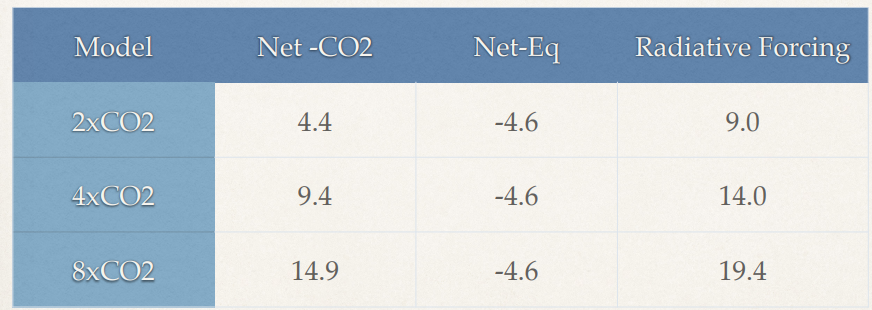
\includegraphics[width=0.5\linewidth]{uploads/image11.png}
	\caption{Black body curves for the solar radiation and the terrestrial radiation for the entire atmosphere and the first 11 km of the atmosphere}
	\label{fig:enter-label}
\end{figure}
Much of the fundamental physics governing radiation transfer is embodied in the following two laws:
\begin{itemize}
	\item Lambert's law, which provides a formulation for the decrease in intensity of radiation of a given wavelength as the radiation passes through a given amount of absorbing gas
	      $$\frac{d}{dz}[I]=Ik\rho$$
	      where k is the absorption coefficient, $\rho$ is the density of the layer, and I is the radiance, defined as the energy per unit time per  unit area per unit solid angle $d\omega$

	\item Kirchhoff's law, states that there is a proportionality between radiative absorptivity and emissivity of a gas at the same temperature for any wavelength. A good absorber of radiation at some wavelength is also a good emitter of radiation at the same wavelength.

	      In particular, it is usually identified absorptivity is the ratio of the amount of radiative energy absorbed to the total incident radiation, and emissivity is the ratio of the emitted radiation to the maximum possible emitted radiation at the same temperature.
\end{itemize}

The formula above shows the relationship between intensity from some given direction, unit solid angle do, and the surface, such that integration over $\theta$ of the hemisphere above the horizontal surface yields the flux, F, arriving from all angles

\begin{equation}\label{eq 2}
	\int(Icos\theta )\,d\omega
\end{equation}

Dividing \ref{eq 2} by I and forming integrals over optical depth on either side yield
$$\int \frac{dI}{I} = - \int k \rho \, dz$$ which becomes $$\ln \left( \frac{I}{I_0} \right) = - \int k \rho \, dz$$
upon integrating the left-hand side.
This can be written exponentially as $$I = I_0 e^{-\chi}$$
where $\chi$ is the optical depth or optical pathlength and $$\tau = e^{-\chi}$$
is the frictional transmission, indicating the fraction of the original radiance that get transmitted to optical depth within attenuating gas.

For a blackbody, the emission is also described by Lambert's law with a different sign
\begin{equation}\label{eq3}
	dI = B(T) k \rho \, dz
\end{equation}

If I integrate \ref{eq3} over a hemisphere, I obtain the Stefan-Boltzmann law
$$\int_0^{2\pi} B(T) \cos \theta \, d\omega = \sigma T^4$$
or $$\pi B(T) = \sigma T^4$$

The change of radiance at a point z is made up of two fluxes
$$\frac{1}{\rho} \frac{dI}{dz} = -k (I - B(T))$$ where kI is the absorption and kB(T) is the emission.
So the fractional absorption in a layer (z,z_1) is $$\tau(z, z_1) = \exp \left( - \int_{z_1}^z k \rho \, dz' \right)$$

\begin{figure}[h!]
	\centering
	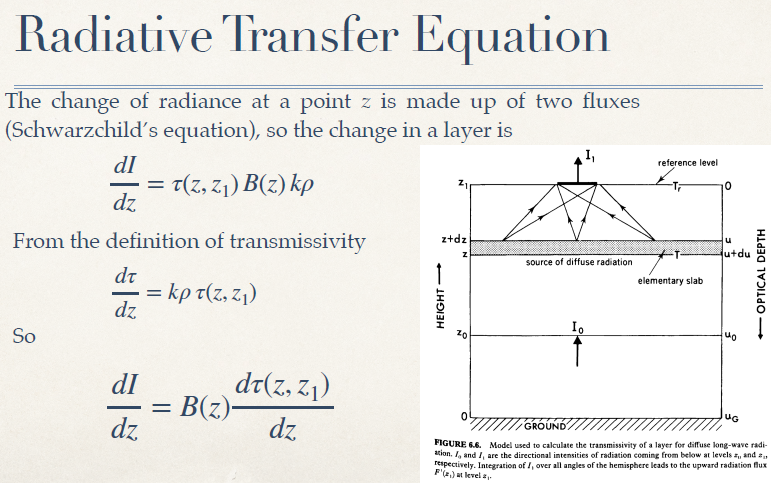
\includegraphics[width=0.5\linewidth]{uploads/16image.png}
	\caption{Enter Caption}
	\label{fig:enter-label}
\end{figure}

\begin{figure}[h!]
	\centering
	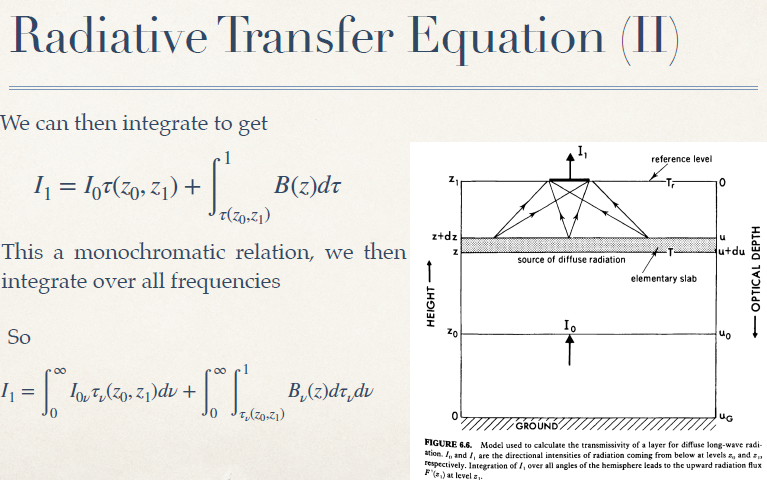
\includegraphics[width=0.5\linewidth]{uploads/17image.png}
	\caption{Enter Caption}
	\label{fig:enter-label}
\end{figure}

\begin{figure}[h!]
	\centering
	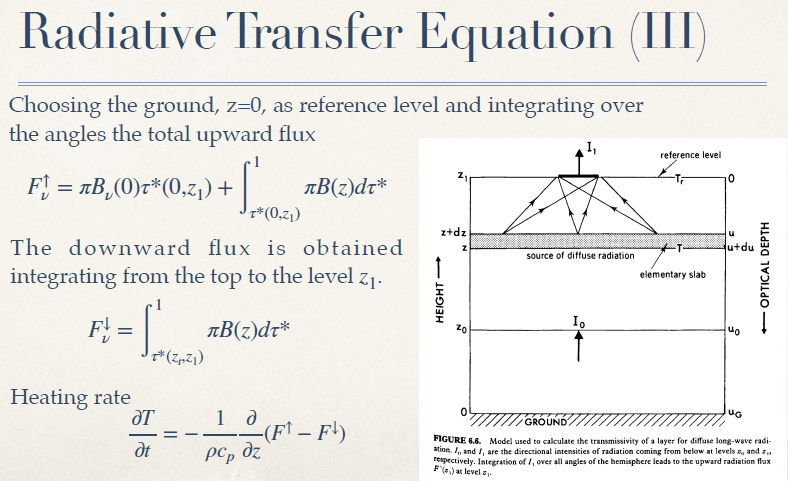
\includegraphics[width=0.5\linewidth]{uploads/18image.png}
	\caption{Enter Caption}
	\label{fig:enter-label}
\end{figure}

The solar radiation is a function of the zenith angle
$$\cos Z = \sin \varphi \sin \delta + \cos \varphi \cos \delta \cos H$$

where $\phi$ is latitude, $\delta$ is solar declination, which is the angular distance of the sun north of the equator and varies from about 23.5° on June 22 to -23.5° on December 22 and H is the hour angle, which is the longitudinal distance from the point in question to the meridian of solar noon and therefore is 0 at any point experiencing solar noon.
The solar flux, S, entering at the top of the atmosphere is a function of cos Z and the distance from the sun to the Earth, d, such that
$$S = S_0 f(d) \cos Z$$
where S_{0} is the so-called solar constant (the solar energy flux received at the outer atmosphere on a surface normal to the solar beam; known now not to be constant) and the factor f(d) is 1.0344 in early January and 0.9674 in July for the present astronomical conditions.
\begin{figure}[h!]
	\centering
	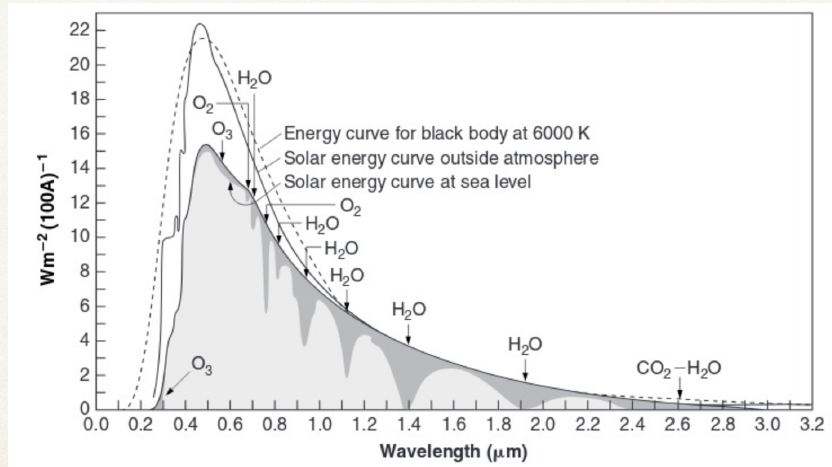
\includegraphics[width=0.5\linewidth]{uploads/image12.png}
	\caption{Spectral energy distribution as a function of wavelength at the top of the atmosphere and at sea level. The figure includes absorption by various atmospheric gases}
	\label{fig1}

\end{figure}
As shown in \ref{fig1} the principal absorber in the atmosphere is the stratospheric ozone, which absorbs very effectively in the ultraviolet and in the visible. Water vapor is the primary absorber in the troposphere in the near-infrared, also with carbon dioxide are the main important absorbers for the longer wavelengths.

\begin{figure}[h!]
	\centering
	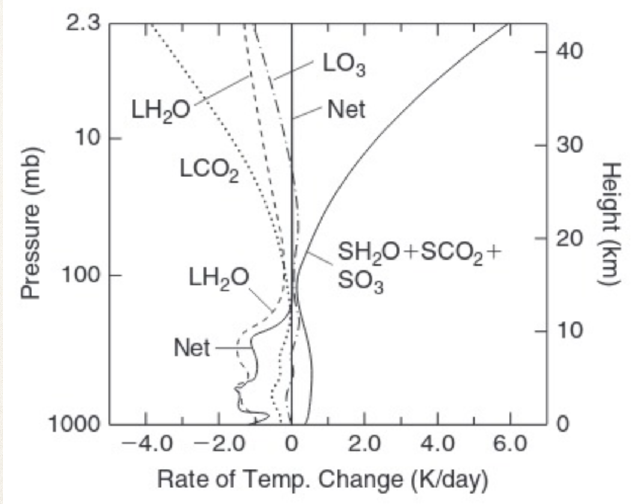
\includegraphics[width=0.5\linewidth]{uploads/image13.png}
	\caption{Heating rates in the atmosphere due to the absorption of solar radiation by atmospheric gases and due to the longwave or infrared radiation}
	\label{figl}
\end{figure}
The largest contributors to the eating/cooling rates are water vapor, carbon dioxide and ozone as shown in Figure \ref{figl}.
The net heating/cooling is zero in the stratosphere because in the one-dimensional model, it is in radiative equilibrium. The troposphere shows a net radiative cooling that is compensated by the vertical transfer of sensible and latent heat from below by moist adiabatic convection. As suggested in Figure \ref{figl} water vapor is the strongest contributor to the troposphere cooling. In the stratosphere cooling due to water vapor, carbon dioxide and ozone is generally compensated by heating due to absorption of solar radiation by zone.

\section{Moisture}
It is the quantity of water vapor in the air and it can be specified in several ways, depending on which reference is used
\begin{itemize}
	\item \textit{mixing ratio} ratio of the density of water vapor to the density of dry air
	\item \textit{specific humidity} ratio concerning the density of moist air
	\item \textit{relative humidity} ratio of the mixing ratio to the saturation mixing ratio
\end{itemize}
The same as the continuity mass treatment, the changes in the amount of water vapor must be balanced by the moisture sources and sinks
\begin{equation}\label{eq3}
	\frac{\partial (\rho q)}{\partial t} + \nabla \cdot (\rho q \vec{v}) + \frac{\partial}{\partial z} (\rho q w) = M + \rho E
\end{equation}

where M is the time rate change of water vapor per unit volume due to condensation or freezing (sinks of moisture) and E is the time rate of change of water vapor content per unit mass due to evaporation from the surface and sub-grid vertical and horizontal diffusion of moisture within the atmosphere (source of moisture).
Often \ref{eq3} is written in flux form by combining with the continuity equation to obtain

\begin{equation}\label{eq4}
	\frac{\partial (\rho q)}{\partial t} + \nabla \cdot (\rho q \vec{V}) + \frac{\partial (\rho q \omega)}{\partial z} = M + \rho E
\end{equation}

If \ref{eq4} is integrated over the entire volume of the atmosphere, the second and the third terms on the left drop out, so that the sources and sinks of moisture must balance to have no secular change in atmospheric moisture over the globe.
If the atmosphere is saturated with moisture, then sensible heat can be added to the atmospheric system from latent heat by the conversion of water vapor to liquid warmer or ice parcels.

The first law of thermodynamic must incorporate in the nonadiabatic term, this energy conversion process due to phase changes between liquid, solid, and gas.
If the nonadiabatic process of conversion of water vapor to liquid water is the only energy source incorporated, the first law of thermodynamics becomes
$$c_p \, dT + \frac{1}{\rho} \, dp = - L \, dqs$$
The equation of state can be written like $$e = \rho_{W} RT$$ where e is the partial pressure for water vapor
Substituting in the previous equation, the mixing ratio becomes now
\begin{equation}\label{eq2}
	q\approx 0.622 \frac{e}{p}
\end{equation}

Inserting a total differential form of the hydrostatic equation, the first law of thermodynamics becomes $$\frac{dT}{dz} = - \frac{g}{c_p} - \frac{L}{c_p} \frac{dqs}{dz}$$
taking the log and differentiating the previous equation \ref{eq2} we will obtain
$$\log q_s \approx \log 0.622 + \log e_s - \log p$$
$$\frac{1}{e_s} \frac{d e_s}{d z} = \frac{1}{q_s} \frac{d q_s}{d z} + \frac{1}{p} \frac{d p}{d z}$$
$$\frac{1}{e_s} \frac{d e_s}{d T} = \frac{1}{q_s} \frac{d q_s}{d z} - \frac{1}{p} g \rho$$

The Clausius-Clapeyron equation relates the change in saturation vapor pressure to the latent heat involved in a phase change from water vapor to liquid water or from liquid water to ice. The most convenient form of this is $$\frac{1}{e_s} \frac{d e_s}{d T} = \frac{L}{R T^2}$$
So we get $$\frac{d q_s}{d z} = \frac{L q_s}{R W T_2} \frac{d T}{d z} + \frac{g q_s}{R T}$$

$$\frac{dT}{dz} = -\frac{g}{c_p} \left( 1 + \frac{L q_s}{R T} \right) \left( 1 + \frac{L^2 q_s}{c_p R W T_2} \right)^{-1}$$
In this way, we will obtain the moist adiabatic lapse rate $\Gamma$, which is less than the adiabatic lapse rate defined earlier

\section{Clouds}
They play a critical role in the radiation characteristics of the Earth's climate, but their radiative properties are not fully understood. In most climate models, the precipitation and convective aspects of the model are used to compute where clouds exist based on whether the atmosphere is near saturation and whether convection is occurring. You can use different parameters to explain that.

\subsection{Cumulus formation}
If a parcel of air near the Earth's surface (at an atmospheric pressure of approximately 1000 mb) starts to rise, say from strong heating, it will cool at approximately the dry adiabatic lapse rate of 9.8 Kkm-¹. When the parcel cools sufficiently the parcel is saturated, gaining a condition of instability because there is much more energy in the water vapor. The level at which this occurs is termed the lifting condensation level, LCL, and is typically at the cloud base as the picture below shows.
\begin{figure}[h!]
	\centering
	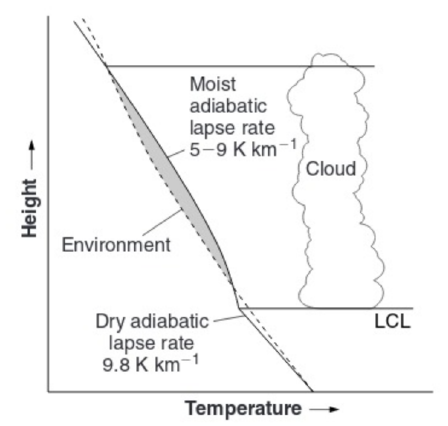
\includegraphics[width=0.5\linewidth]{uploads/image14.png}
	\caption{Enter Caption}
	\label{fig:enter-label}
\end{figure}
If the parcel does not rise high enough to reach an LCL, then a cloud should not form. From the LCL upward, the parcel will cool less rapidly as it rises since the latent heat of condensation or fusion releases heat. This lessened rate of temperature decrease with height is the moist adiabatic lapse rate.

\begin{figure}[h!]
	\centering
	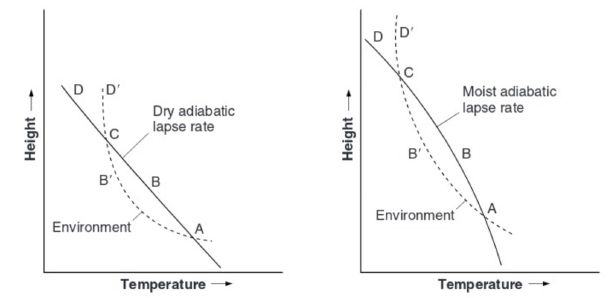
\includegraphics[width=0.5\linewidth]{uploads/image15.png}
	\caption{Diagram of stable and unstable conditions concerning dry and moist lapse rates.}
	\label{fig: figure 15}
\end{figure}
As shown in figure \ref{fig: figure 15} the dotted curve represents conditions for the environmental air, and the solid curves represent conditions for the path along which a parcel will ascend from point A to B, depending on whether the dry or the moist adiabatic lapse rate is appropriate. There is a point B' highlighted on the curve for the environmental air that is colder in both cases than point B for the parcel at the same height. Since the air at B' is colder than that at B, the parcel will have positive buoyancy. Thus in principle, it will continue ascending. If on the other hand, a parcel is at C and ascends to point D, it will be colder than the surrounding environmental air at D'. Thus the parcel will have negative buoyancy, which will cause it to sink to its original position.

\section{Surface Processes}
Boundary fluxes for momentum and heat, we can physically represent as
$$\tau_x = \rho C_D \left| \vec{v} - \vec{v_s} \right| (u_s - u)$$
$$\tau_y = \rho C_D \left| \vec{v} - \vec{v_s} \right| (v_s - v)$$
$$H = \rho c_p C_H \left| \vec{v} - \vec{v_s} \right| (\theta_s - \theta)$$
$$LE = \rho L_C E \left| \vec{v} - \vec{v_s} \right| (q_s - q)$$

Where over land $\vec{v}$ is zero.

Above the surface boundary layer adjacent to Earth's surface exists the planetary boundary layer, where the wind turns with the height. Within this region, the balance of forces can be approximated by Coriolis, pressure gradient, and frictional forces through the following simplification
$$-f_{\nu} = - \frac{1}{\rho a \cos \varphi} \frac{\partial p}{\partial \lambda} + F_{\lambda}$$
$$f_u = - \frac{1}{\rho a} \frac{\partial p}{\partial \varphi} + F_{\varphi}$$

The frictional term can be expressed as the vertical gradient of stress, so that $$F_\lambda = \frac{1}{\rho} \frac{\partial \tau_\lambda}{\partial z}$$
and $$F_\varphi = \frac{1}{\rho} \frac{\partial \tau_\varphi}{\partial z}$$


and the stress can in turn be related to the vertical gradient of wind shear
$$\tau_\lambda = \rho K_m \frac{\partial u}{\partial z}$$
and $$\tau_\varphi = \rho K_m \frac{\partial v}{\partial z}$$

where Km is the vertical eddy or transfer coefficient for momentum. Note that if the vertical wind shear is large, as one would expect near the Earth's surface since the wind must approach zero at the surface, then the momentum transfer is also large. On the molecular scale, Km, takes on values appropriate for those space scales; however, in the atmosphere and ocean models the space scales are much larger. Many of the eddies have dimensions of the order of the spatial grid structure of the models.
If the layer is unstable there is strong vertical mixing and Km is large; if the layer is stable there is no strong coupling and Km is small. A useful measure of this stability is the Richardson number Ri, which is defined as
$$R_i = \frac{g}{\theta} \frac{\frac{\partial \theta}{\partial z}}{\left( \frac{\partial V}{\partial z} \right)^2}$$
where $V = \left| \vec{V} \right|$ and $\frac{\partial V}{\partial z}$ is the vertical wind shear or vertical gradient of wind velocity.

\section{Hydrology}
\begin{figure}[h!]
	\centering
	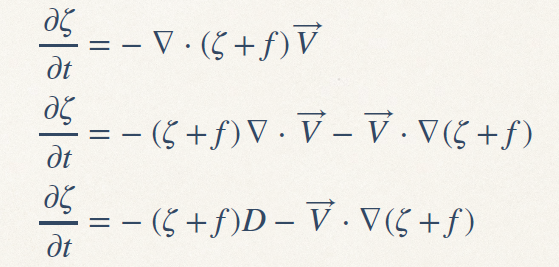
\includegraphics[width=0.5\linewidth]{uploads/15image.png}
	\caption{Schematic processes and features relevant to surface hydrology and evapotraspiration}
	\label{fig: fig 2}
\end{figure}
As shown in \ref{fig: fig 2} lots of processes are involved in surface hydrology. These include radiation, sensible heat, evaporation, transpiration, momentum, and precipitation, but also H2O and CO2 fluxes. The surface moisture can contribute to surface flow in streams percolate to a deeper layer or even become groundwater, depending on the porous properties of the ground. In the root zones of plants, some of the surface moisture can be taken up by the plant roots and then relayed to the plant leaves and transpired.

Within a land area as large as a horizontal grid cell of a global model, there are generally multiple surface types, including lakes, wetlands, different vegetation types, and different soil types
Another aspect of land surface processes being improved in many climate models is the simulation of snow coverage. The snow modeling community has developed a variety of models that can be used for climate and hydrology. These models range from the simple to the complex, and several of them are specifically designed for use in general circulation models. The more complex snow models take into account melting processes, grain size, shape, liquid water content, and percolation processes.

